\documentclass[]{article}

\usepackage{tabularx}
\usepackage[dutch]{babel}
\usepackage{amsmath}
\usepackage{graphicx}
\usepackage{amsmath}
\usepackage{epstopdf}
\usepackage[parfill]{parskip}

\newcommand{\opgave}[1]{\section*{Opgave #1}}

\begin{document}

\opgave7


De interlacing eigenschap zegt dat bij een symmetrische tridiagonale matrix $\lambda ^{(k+1)}_{j} < \lambda ^{(k)}_{j} < \lambda ^{(k+1)}_{j+1}$, waarbij $\lambda ^{(k)}_{j}$ de $j^{de}$ eigenwaards is van de $k^{de}$ principiele submatrix. $\lambda _{1}$ is dan de kleinste eigenwaarde van $A^{k}$ en $\lambda _{k}$ de grootste. We zullen deze eigenschap illustreren aan de hand van het volgende voorbeeld.

\begin{equation}
A=\begin{bmatrix}
    	8 & 4 & 0 & 0 & 0	\\
    	4 & 3 & -3 & 0 & 0 \\
    	0 & -3 & 9 & -2 & 0 \\
    	0 & 0 & -2 & 1 & -2 \\
    	0 & 0 & 0 & -2 & 6 
    \end{bmatrix}
    ,
    A^{1}=\begin{bmatrix}
        	8
        \end{bmatrix}
        ,
    A^{2}=\begin{bmatrix}
           	8 & 4 \\
           	4 & 3
         \end{bmatrix}
         , ...
\end{equation}
\begin{figure}
\noindent 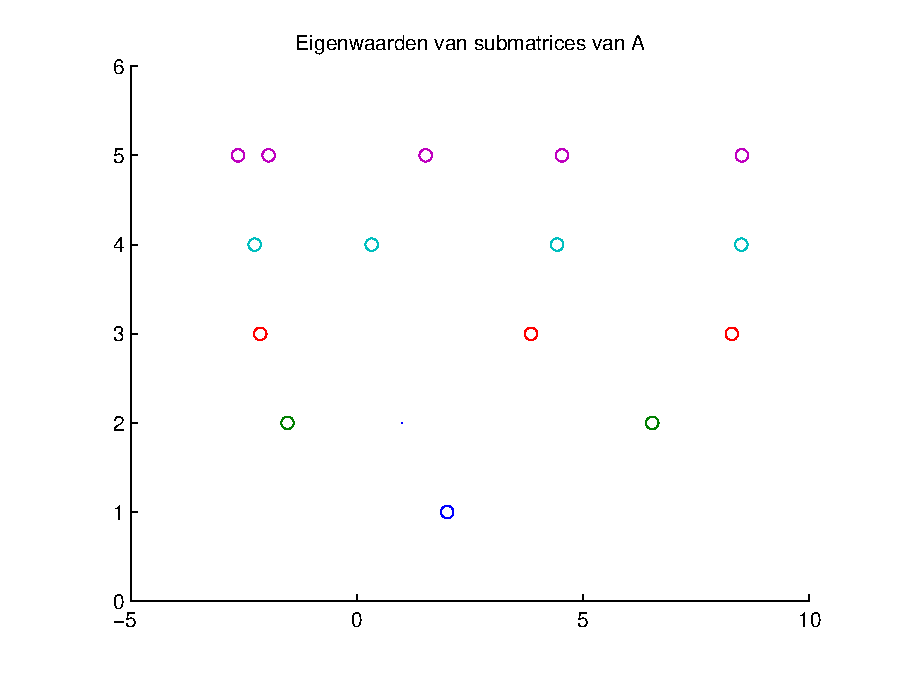
\includegraphics[width=1\linewidth]{opgave7.eps}
\caption{Interlacing}
\label{figuurtje}
\end{figure}

\begin{table}
\noindent\makebox[\textwidth]{%
\begin{tabularx}{0.8\textwidth}{l|llllll}
Submatrix&$\lambda _{1}$&$\lambda _{2}$&$\lambda _{3}$&$\lambda _{4}$&$\lambda _{5}$\\\hline
$A^{1}$&$2$ & $/$ & $/$ & $/$ & $/$ \\
$A^{2}$&$-1.5311$ & $6.5311$ & $/$ & $/$ & $/$\\
$A^{3}$&$-2.1330$ & $3.8478$ & $8.2852$ & $/$ & $/$\\
$A^{4}$&$-2.2544$ & $.30192$ & $4.4261$ & $8.4980$ & $/$\\
$A^{5}$&$-2.6223$ & $-1.9468$ & $1.5220$ & $4.5360$ & $8.5111$\\
\end{tabularx}}
\caption{Eigenwaarden van de principiele submatrices van A}
\label{tabelOpgave4}
\end{table}

Het is duidelijk aan de hand van de bovenstaande tabel dat de interlacing eigenschap geldt. Bijvoorbeeld $-2.1330 < -1.5311 < 3.8478 < 6.5311 < 8.2852$ voor $A^{2}$ en $A^{3}$

\end{document}